\documentclass[tikz, border=20pt]{standalone}
\usepackage{amsmath, amssymb}
\usetikzlibrary{positioning, arrows.meta, calc, shapes.geometric, fit, backgrounds}

\begin{document}
	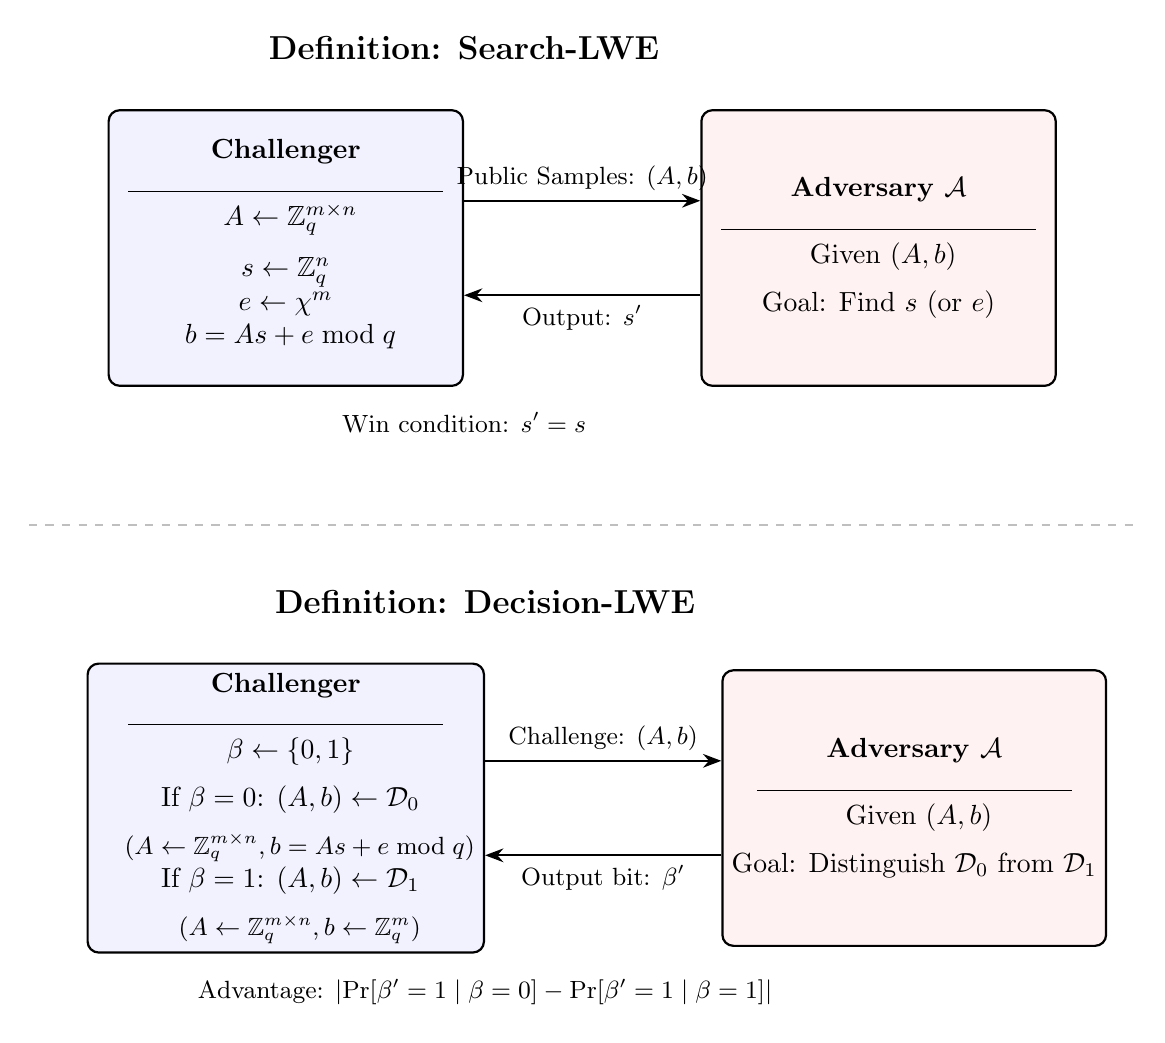
\begin{tikzpicture}[
		>=Stealth,
		node distance=4cm and 3cm,
		entity/.style={draw, thick, rounded corners, minimum height=3.5cm, minimum width=4.5cm, align=center, fill=blue!5},
		adv/.style={draw, thick, rounded corners, minimum height=3.5cm, minimum width=4.5cm, align=center, fill=red!5},
		message/.style={->, thick},
		title/.style={font=\large\bfseries}
		]
		
		% ==========================================
		% DEFINITION 1: SEARCH-LWE
		% ==========================================
		
		\node[entity] (ChallengerS) {
			\textbf{Challenger} \\
			\rule{4cm}{0.4pt} \\ \vspace{0.1cm}
			$A \leftarrow \mathbb{Z}_q^{m \times n}$ \\
			$s \leftarrow \mathbb{Z}_q^n$ \\
			$e \leftarrow \chi^m$ \\ \vspace{0.1cm}
			$b = As + e \bmod q$
		};
		
		\node[adv, right=of ChallengerS] (AdvS) {
			\textbf{Adversary $\mathcal{A}$} \\
			\rule{4cm}{0.4pt} \\ \vspace{0.1cm}
			Given $(A, b)$ \\
			Goal: Find $s$ (or $e$)
		};
		
		\draw[message] ([yshift=0.6cm]ChallengerS.east) -- node[above, font=\small] {Public Samples: $(A, b)$} ([yshift=0.6cm]AdvS.west);
		\draw[message] ([yshift=-0.6cm]AdvS.west) -- node[below, font=\small] {Output: $s'$} ([yshift=-0.6cm]ChallengerS.east);
		
		% Win Condition S
		\node[below=0.2cm of ChallengerS.south east, anchor=north, font=\small] (WinS) {Win condition: $s' = s$};
		
		\node[above=0.5cm of ChallengerS.north east, anchor=south, title] {Definition: Search-LWE};
		
		% ==========================================
		% DEFINITION 2: DECISION-LWE
		% ==========================================
		
		\node[entity, below=3.5cm of ChallengerS] (ChallengerD) {
			\textbf{Challenger} \\
			\rule{4cm}{0.4pt} \\ \vspace{0.1cm}
			$\beta \leftarrow \{0, 1\}$ \\ \vspace{0.1cm}
			If $\beta = 0$: $(A,b) \leftarrow \mathcal{D}_0$ \\
			\quad {\small ($A \leftarrow \mathbb{Z}_q^{m \times n}, b = As+e \bmod q$)} \\ \vspace{0.1cm}
			If $\beta = 1$: $(A,b) \leftarrow \mathcal{D}_1$ \\
			\quad {\small ($A \leftarrow \mathbb{Z}_q^{m \times n}, b \leftarrow \mathbb{Z}_q^m$)}
		};
		
		\node[adv, right=of ChallengerD] (AdvD) {
			\textbf{Adversary $\mathcal{A}$} \\
			\rule{4cm}{0.4pt} \\ \vspace{0.1cm}
			Given $(A, b)$ \\
			Goal: Distinguish $\mathcal{D}_0$ from $\mathcal{D}_1$
		};
		
		\draw[message] ([yshift=0.6cm]ChallengerD.east) -- node[above, font=\small] {Challenge: $(A, b)$} ([yshift=0.6cm]AdvD.west);
		\draw[message] ([yshift=-0.6cm]AdvD.west) -- node[below, font=\small] {Output bit: $\beta'$} ([yshift=-0.6cm]ChallengerD.east);
		
		% Win Condition D
		\node[below=0.2cm of ChallengerD.south east, anchor=north, font=\small] (WinD) {Advantage: $\left| \Pr[\beta'=1 \mid \beta=0] - \Pr[\beta'=1 \mid \beta=1] \right|$};
		
		\node[above=0.5cm of ChallengerD.north east, anchor=south, title] {Definition: Decision-LWE};
		
		% ==========================================
		% DIVIDER
		% ==========================================
		\draw[dashed, gray!50, thick] ([yshift=-1.75cm, xshift=-1cm]ChallengerS.south west) -- ([yshift=-1.75cm, xshift=1cm]AdvS.south east);
		
	\end{tikzpicture}
\end{document}